\documentclass{article}
\usepackage[margin=2cm]{geometry}

\input{./basic-tex-config/preamble.tex}

\graphicspath{{./images/}}

\title{ЛАБОЛАТОРНАЯ РАБОТА ПО КУРСУ\\ <<КВАНТОВЫЙ КОМПЬЮТЕР>>\\
Однокубитовые квантовые схемы}
\date{Санкт-Петербург, 2017}
\author{Плотников Антон, А4101}

\begin{document}

\maketitle
\newpage

\section{Цель работы}
Изучение простейших однокубитовых квантовых логических схем.

\section{Задачи}

\begin{enumerate}
  \item Изучение работы квантовых логических схем, составленных из
    элементов алгоритмов X, Z и H.

  \item Прогнозирование результатов виртуального эксперимента и сравнение
    результатов теоретических и экспериментальных расчетов.
\end{enumerate}

\section{Методика проведения исследования}

Выбираем несколько квантовых элементов, подаем на вход цепочки элементов кубит.
Используя матричное представление схемы, сравниваем результаты теоретических
расчетов с полученными экспериментальными данными.

\section{Анализ погрешностей}

Пусть $\ket{\phi1}$ – состояние, соответствующее первой альтернативе, а
$\ket{\phi2}$ – состояние, соответствующее второй альтернативе. Пусть перед
измерением система находилась в состоянии $c_1\ket{\phi1} + c_2\ket{\phi2}$.
Тогда с вероятностью $\ket{c_1|^2$ измерение даст первый результат, и система
окажется после измерения в состоянии $|\phi1}$, а с вероятностью $\ket{c_2|^2$
измерение даст второй результат, и система окажется после измерения в состоянии
$|\phi2}$.

Таким образом, при измерении исходного состояния $\ket{\phi} =
0.412\ket{0}+0.911\ket{1}$ с вероятностью $p\approx0.17$ мы получим $\ket{0}$ и
с вероятностью $p\approx0.83$ - $\ket{1}$.

\section{Результаты}

 Исходный вектор: $\ket{\phi} = 0.412\ket{0}+0.911\ket{1}$

\subsection{U=XZH}

Теоретические расчеты:
\begin{equation}
  XZH\begin{pmatrix} \alpha\\ \beta \end{pmatrix} = \begin{pmatrix} 0 & 1 \\ 1
                                                                      &
  0\end{pmatrix}\begin{pmatrix}\begin{array}{rr} 1 & 0 \\ 0 & -1 \end{array}
  \end{pmatrix}\frac{1}{\sqrt{2}}\begin{pmatrix}\begin{array}{rr} 1 & 1 \\ 1 &
  -1 \end{array} \end{pmatrix}\begin{pmatrix} 0.412 \\
  0.911\end{pmatrix}\approx\begin{pmatrix} 0.353\\0.935 \end{pmatrix}
  \end{equation}

Экспериментальные расчеты:

\begin{figure}[H]
	\center{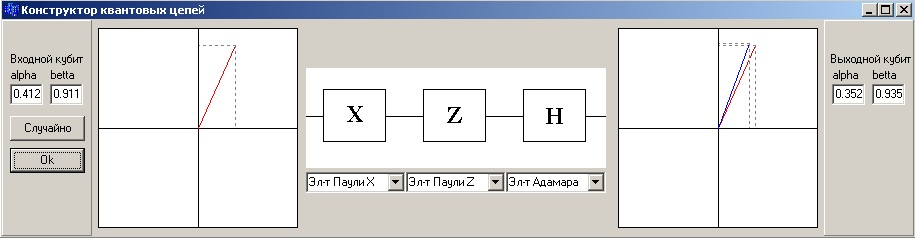
\includegraphics[width=0.85\textwidth]{XZH}}
\end{figure}


\subsection{U=ZZH}

Теоретические расчеты:
\begin{equation}
  ZZH\begin{pmatrix} \alpha\\ \beta \end{pmatrix} =
  \begin{pmatrix}\begin{array}{rr} 1 & 0 \\ 0 & -1 \end{array}
  \end{pmatrix}\begin{pmatrix}\begin{array}{rr} 1 & 0 \\ 0 & -1 \end{array}
  \end{pmatrix}\frac{1}{\sqrt{2}}\begin{pmatrix}\begin{array}{rr} 1 & 1 \\ 1 &
  -1 \end{array} \end{pmatrix}\begin{pmatrix} 0.412 \\ 0.911
  \end{pmatrix}=I\frac{1}{\sqrt{2}}\begin{pmatrix} \begin{array}{rr}1 & 1 \\
  1 & -1 \end{array}\end{pmatrix}\begin{pmatrix} 0.412 \\ 0.911
  \end{pmatrix}\approx\begin{pmatrix} \begin{array}{r}0.935\\-0.353
  \end{array}\end{pmatrix}
\end{equation}

 Экспериментальные расчеты:

 \begin{figure}[H]
	\center{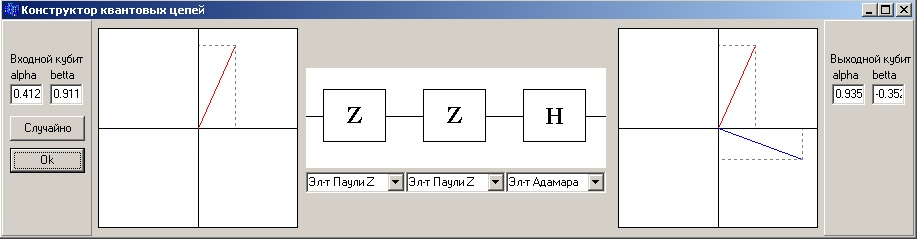
\includegraphics[width=0.85\textwidth]{ZZH}}
\end{figure}

\subsection{U=XXX}

Теоретические расчеты:
\begin{equation}
  XXX\begin{pmatrix} \alpha\\ \beta \end{pmatrix} = X\begin{pmatrix} \alpha\\
  \beta \end{pmatrix}=\begin{pmatrix} 0 & 1 \\ 1 & 0
  \end{pmatrix}\begin{pmatrix} 0.412 \\ 0.911 \end{pmatrix}=\begin{pmatrix}
  0.911\\0.412 \end{pmatrix}
\end{equation}

Экспериментальные расчеты:

\begin{figure}[H]
	\center{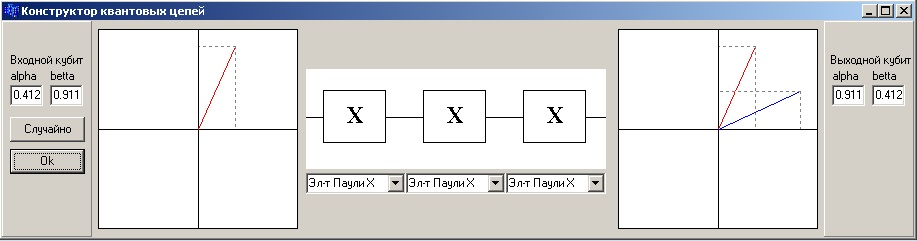
\includegraphics[width=0.85\textwidth]{XXX}}
\end{figure}

\section{Выводы}

Изучив работу квантовых логических схем, составленных из элементов алгоритмов
X, Z и H, сравнили результаты теоретических и экспериментальных расчетов. В
результате получили одинаковые результаты, за исключением погрешности
округления. Также проверили утверждение, что $UU=I$ и $UUU=U$.

\end{document} 
